% Created by tikzDevice version 0.12.4 on 2025-05-16 12:48:15
% !TEX encoding = UTF-8 Unicode
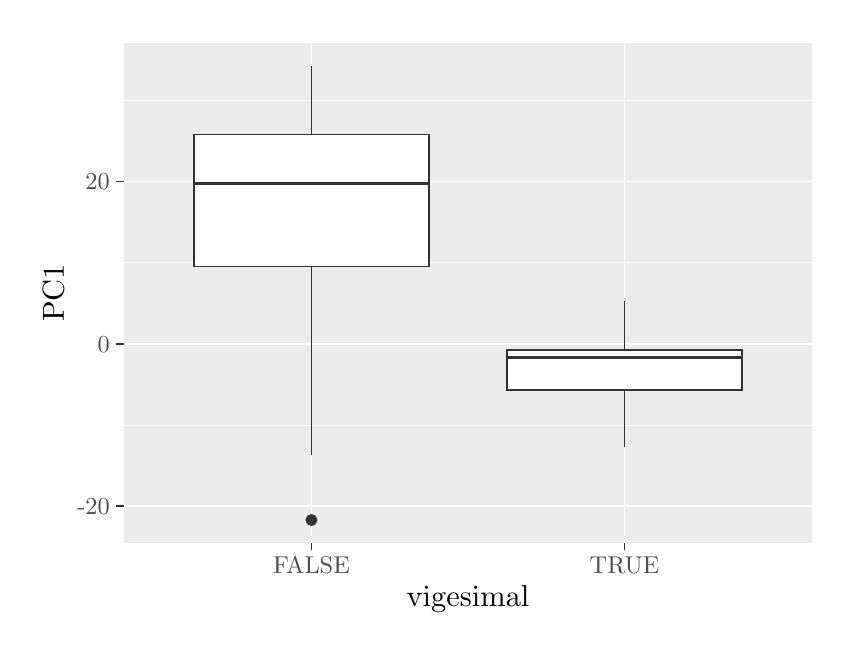
\begin{tikzpicture}[x=1pt,y=1pt]
\definecolor{fillColor}{RGB}{255,255,255}
\path[use as bounding box,fill=fillColor,fill opacity=0.00] (0,0) rectangle (289.08,216.81);
\begin{scope}
\path[clip] (  0.00,  0.00) rectangle (289.08,216.81);
\definecolor{drawColor}{RGB}{255,255,255}
\definecolor{fillColor}{RGB}{255,255,255}

\path[draw=drawColor,line width= 0.6pt,line join=round,line cap=round,fill=fillColor] (  0.00,  0.00) rectangle (289.08,216.81);
\end{scope}
\begin{scope}
\path[clip] ( 34.64, 30.69) rectangle (283.58,211.31);
\definecolor{fillColor}{gray}{0.92}

\path[fill=fillColor] ( 34.64, 30.69) rectangle (283.58,211.31);
\definecolor{drawColor}{RGB}{255,255,255}

\path[draw=drawColor,line width= 0.3pt,line join=round] ( 34.64, 73.23) --
	(283.58, 73.23);

\path[draw=drawColor,line width= 0.3pt,line join=round] ( 34.64,131.87) --
	(283.58,131.87);

\path[draw=drawColor,line width= 0.3pt,line join=round] ( 34.64,190.51) --
	(283.58,190.51);

\path[draw=drawColor,line width= 0.6pt,line join=round] ( 34.64, 43.91) --
	(283.58, 43.91);

\path[draw=drawColor,line width= 0.6pt,line join=round] ( 34.64,102.55) --
	(283.58,102.55);

\path[draw=drawColor,line width= 0.6pt,line join=round] ( 34.64,161.19) --
	(283.58,161.19);

\path[draw=drawColor,line width= 0.6pt,line join=round] (102.54, 30.69) --
	(102.54,211.31);

\path[draw=drawColor,line width= 0.6pt,line join=round] (215.69, 30.69) --
	(215.69,211.31);
\definecolor{drawColor}{gray}{0.20}
\definecolor{fillColor}{gray}{0.20}

\path[draw=drawColor,line width= 0.4pt,line join=round,line cap=round,fill=fillColor] (102.54, 38.90) circle (  1.96);

\path[draw=drawColor,line width= 0.6pt,line join=round] (102.54,178.20) -- (102.54,203.10);

\path[draw=drawColor,line width= 0.6pt,line join=round] (102.54,130.56) -- (102.54, 62.34);
\definecolor{fillColor}{RGB}{255,255,255}

\path[draw=drawColor,line width= 0.6pt,fill=fillColor] ( 60.10,178.20) --
	( 60.10,130.56) --
	(144.97,130.56) --
	(144.97,178.20) --
	( 60.10,178.20) --
	cycle;

\path[draw=drawColor,line width= 1.1pt] ( 60.10,160.61) -- (144.97,160.61);

\path[draw=drawColor,line width= 0.6pt,line join=round] (215.69,100.45) -- (215.69,118.02);

\path[draw=drawColor,line width= 0.6pt,line join=round] (215.69, 85.78) -- (215.69, 65.28);

\path[draw=drawColor,line width= 0.6pt,fill=fillColor] (173.26,100.45) --
	(173.26, 85.78) --
	(258.12, 85.78) --
	(258.12,100.45) --
	(173.26,100.45) --
	cycle;

\path[draw=drawColor,line width= 1.1pt] (173.26, 97.50) -- (258.12, 97.50);
\end{scope}
\begin{scope}
\path[clip] (  0.00,  0.00) rectangle (289.08,216.81);
\definecolor{drawColor}{gray}{0.30}

\node[text=drawColor,anchor=base east,inner sep=0pt, outer sep=0pt, scale=  0.88] at ( 29.69, 40.88) {-20};

\node[text=drawColor,anchor=base east,inner sep=0pt, outer sep=0pt, scale=  0.88] at ( 29.69, 99.52) {0};

\node[text=drawColor,anchor=base east,inner sep=0pt, outer sep=0pt, scale=  0.88] at ( 29.69,158.16) {20};
\end{scope}
\begin{scope}
\path[clip] (  0.00,  0.00) rectangle (289.08,216.81);
\definecolor{drawColor}{gray}{0.20}

\path[draw=drawColor,line width= 0.6pt,line join=round] ( 31.89, 43.91) --
	( 34.64, 43.91);

\path[draw=drawColor,line width= 0.6pt,line join=round] ( 31.89,102.55) --
	( 34.64,102.55);

\path[draw=drawColor,line width= 0.6pt,line join=round] ( 31.89,161.19) --
	( 34.64,161.19);
\end{scope}
\begin{scope}
\path[clip] (  0.00,  0.00) rectangle (289.08,216.81);
\definecolor{drawColor}{gray}{0.20}

\path[draw=drawColor,line width= 0.6pt,line join=round] (102.54, 27.94) --
	(102.54, 30.69);

\path[draw=drawColor,line width= 0.6pt,line join=round] (215.69, 27.94) --
	(215.69, 30.69);
\end{scope}
\begin{scope}
\path[clip] (  0.00,  0.00) rectangle (289.08,216.81);
\definecolor{drawColor}{gray}{0.30}

\node[text=drawColor,anchor=base,inner sep=0pt, outer sep=0pt, scale=  0.88] at (102.54, 19.68) {FALSE};

\node[text=drawColor,anchor=base,inner sep=0pt, outer sep=0pt, scale=  0.88] at (215.69, 19.68) {TRUE};
\end{scope}
\begin{scope}
\path[clip] (  0.00,  0.00) rectangle (289.08,216.81);
\definecolor{drawColor}{RGB}{0,0,0}

\node[text=drawColor,anchor=base,inner sep=0pt, outer sep=0pt, scale=  1.10] at (159.11,  7.64) {vigesimal};
\end{scope}
\begin{scope}
\path[clip] (  0.00,  0.00) rectangle (289.08,216.81);
\definecolor{drawColor}{RGB}{0,0,0}

\node[text=drawColor,rotate= 90.00,anchor=base,inner sep=0pt, outer sep=0pt, scale=  1.10] at ( 13.08,121.00) {PC1};
\end{scope}
\end{tikzpicture}
